\documentclass{beamer}
\usepackage[ngerman]{babel}
\usepackage[utf8]{inputenc}
\usetheme{Boadilla}

\begin{document}
\title{Dualcode}
\subtitle{Grundlagenfach Informatik}
%\subtitle{Freifach Informatik}
%\subtitle{Berufsfeldfach Informatik}
%\subtitle{Ergänzungsfach Informatik}
\author{Oliver Probst (pro@kwse.ch)}
\institute{KSWE}
\date{18. August 2022}
\titlegraphic{
\includegraphics[scale=0.5]{graphics/kswe_logo.pdf}}

\begin{frame}
\titlepage
\end{frame}

\frame[c]{\frametitle{Ziel}
\begin{center}
Wie kann man eine natürliche Zahl mithilfe von Binärziffern darstellen?
\end{center}

}

%https://www.inf-schule.de/kids/datennetze/Binaerzahlen/schritt4

\frame[c]{\frametitle{Zaubertrick...}\framesubtitle{Start}
\begin{center}
Wählen Sie eine Zahl zwischen $0$ und $63$. \\ Schreiben Sie die Zahl auf ein Papier.
\end{center}
}

\frame[c]{\frametitle{Zaubertrick...}\framesubtitle{Blatt 1}
\begin{figure}
\centering
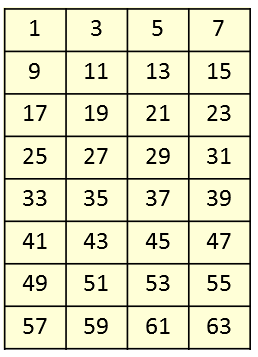
\includegraphics[scale=0.9]{graphics/zaubertrick_1}
\end{figure}
}

\frame[c]{\frametitle{Zaubertrick...}\framesubtitle{Blatt 2}
\begin{figure}
\centering
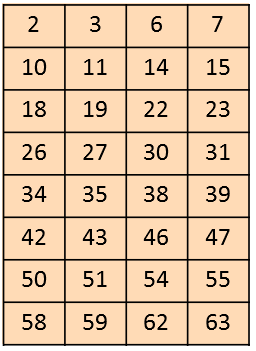
\includegraphics[scale=0.9]{graphics/zaubertrick_2}
\end{figure}
}

\frame[c]{\frametitle{Zaubertrick...}\framesubtitle{Blatt 3}
\begin{figure}
\centering
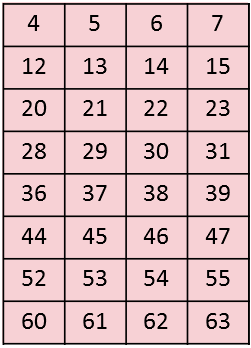
\includegraphics[scale=0.9]{graphics/zaubertrick_3}
\end{figure}
}

\frame[c]{\frametitle{Zaubertrick...}\framesubtitle{Blatt 4}
\begin{figure}
\centering
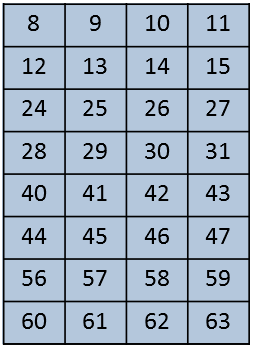
\includegraphics[scale=0.9]{graphics/zaubertrick_4}
\end{figure}
}

\frame[c]{\frametitle{Zaubertrick...}\framesubtitle{Blatt 5}
\begin{figure}
\centering
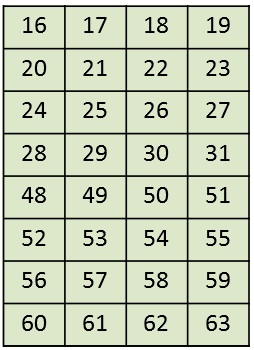
\includegraphics[scale=0.9]{graphics/zaubertrick_5}
\end{figure}
}

\frame[c]{\frametitle{Zaubertrick...}\framesubtitle{Blatt 6}
\begin{figure}
\centering
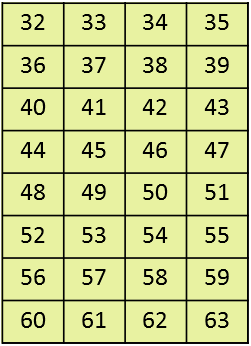
\includegraphics[scale=0.9]{graphics/zaubertrick_6}
\end{figure}
}

\frame[c]{\frametitle{Codes: Dualcode}\framesubtitle{Codieren: Dezimalzahl $\Rightarrow$ Dualzahl}

}

\frame[c]{\frametitle{Codes: Dualcode}\framesubtitle{Decodieren: Dualzahl $\Rightarrow$ Dezimalzahl}

}

\end{document}